\nsection{Problem 3 - (Bayesian Approach)}
Assuming that the data $Y_i$ are on the same form as in Exercise 1, i.e.
$$
y_i=\beta_i+\varepsilon_i, i=1, \ldots, n,
$$
where the parameters are as described for (1). Assume also that $y_i$, follows the mixture distribution as in Exercise 2,
$$
f\left(y_i\right)=p \cdot \phi\left(y_i ; 0,1^2\right)+(1-p) \cdot \phi\left(y_i ; 0, \tau^2+1^2\right)
$$
\nssection{a.)}
\emph{Use a Bayesian interpretation of $\beta_i$, (e.g. assume $\beta_i$ is random) and argue that $\mathbb{P}\left(\beta_i=0 \mid C_i=0\right)=1$, and that $f\left(\beta_i \mid C_i=1\right)=\phi\left(\beta_i ; 0, \tau^2\right)$. Give an expression for $\mathbb{P}\left(\beta_i=0 \mid y_i=y\right)$.}  \spaze
\textbf{Solution:} \spaze
\begin{itemize}
    \item \textbf{Result 1: $\mathbb{P}\left(\beta_i=0 \mid C_i=0\right)=1$}
\end{itemize}
By construction of our model we have that 
\begin{align}
    Y_i = \beta_i + \varepsilon_i 
\end{align}
whereby looking at the conditionals with respect to $C_i = 0$ yields
\begin{align}
Y_i|(C_i = 0) = \beta_i|(C_i=0) + \varepsilon_i|(C_i=0) \label{eq:cond_eq}
\end{align}
But the $\varepsilon_i$ are by assumption independent of the class/mode, and moreover standard normal distributed variables (i.e $\varepsilon_i \sim \mathcal{N}(0,1)$) meaning thus that both the right and left hand sides of Eq.(\ref{eq:cond_eq}) must follow a standard normal distribution with mean $\beta_i|(C_i=0)$ and variance $1$. Since $\beta_i$ and $\varepsilon_i$ are independent it follows that $\mathbb{P}(\beta_i=0 | C_i =0) = 1$.
\begin{itemize}
    \item \textbf{Result 2: $f\left(\beta_i \mid C_i=1\right)=\phi\left(\beta_i ; 0, \tau^2\right)$} 
\end{itemize}
In like manner we have that 
\begin{align} 
    Y_i|(C_i = 1) = \beta_i|(C_i=1) + \varepsilon_i|(C_i=1)  \label{eq:cond_eq2}
\end{align}
where again $\varepsilon_i$ are assumed to be independent of the class/mode. Since we now are conditioning on the class/mode $C_i = 1$, and know that $\beta_i$ and $\varepsilon_i$ are independent, it follows that the only distribution satisfying Eq.(\ref{eq:cond_eq2}) is $\beta_i | (C_i = 1) \sim \mathcal{N}(0, \tau^2)$ since 
\begin{align*}
    f(y_i|C_i=1) &= f(\beta_i + \varepsilon_i| C_i = 1)  \Rightarrow  \boxed{f(y_i|C_i=1) \sim \mathcal{N}(0, \tau^2 + 1)} \\[5pt]
    &=  f(\beta_i |C_i=1) + f(\varepsilon_i | C_i = 1) \\[5pt]
    &= f(\beta_i |C_i=1) + \mathcal{N}(0, 1) \\[5pt]
    &= \mathcal{N}(0, \tau^2) + \mathcal{N}(0, 1) \\[5pt]
    &= \mathcal{N}(0, \tau^2 + 1).
\end{align*}
To express $\mathbb{P}\left(\beta_i=0 \mid y_i=y\right)$ we rewrite it as
\begin{align}
     \mathbb{P}\left(\beta_i=0 \mid y_i=y\right) &= \mathbb{P}(\beta_i = 0 | C_i=0, y_i=y) \mathbb{P}(C_i =0| y_i=y) \\
     &+ \mathbb{P}(\beta_i =0| C_i =1, y_i=y) \mathbb{P}(C_i =1| y_i=y) \label{eq:full_cond}
\end{align}
where we have used the law of total probability \footnote{$P(A) = \sum_{i} P(A | B_i) \cdot P(B_i)$}. Further, we apply Bayes´ rule on the complete expression Eq.(\ref{eq:full_cond})
\begin{align*}
\mathbb{P}\left(\beta_i=0 \mid y_i=y\right) &= \mathbb{P}(\beta_i = 0 | C_i=0, y_i=y) \cdot \frac{\mathbb{P}(y_i=y|C_i=0) \cdot \mathbb{P}(C_i=0)}{\mathbb{P}(y_i=y)} \\ 
&+ \mathbb{P}(\beta_i =0| C_i =1, y_i=y) \cdot \frac{\mathbb{P}(y_i=y|C_i=1) \cdot \mathbb{P}(C_i=1)}{\mathbb{P}(y_i=y)} \\[8pt]
&= \frac{\mathbb{P}(y_i=y|\beta_i=0, C_i=0) \cdot \mathbb{P}(\beta_i=0|C_i=0) \cdot \mathbb{P}(C_i=0)}{\mathbb{P}(y_i=y)} \\
&+ \frac{\mathbb{P}(y_i=y|\beta_i=0, C_i=1) \cdot \mathbb{P}(\beta_i=0|C_i=1) \cdot \mathbb{P}(C_i=1)}{\mathbb{P}(y_i=y)} 
\end{align*}
where we then assume $y_i = \beta_i + \varepsilon_i$ and independence on $\beta_i$ and $\varepsilon_i$, giving
\begin{align*}
    \mathbb{P}\left(\beta_i=0 \mid y_i=y\right) &= \mathbb{P}(\varepsilon_i = y) \cdot \frac{1 \cdot \mathbb{P}(C_i=0)}{\mathbb{P}(y_i = y)} + 0 \cdot \frac{\mathbb{P}(y_i=y|\beta_i=0, C_i=1) \cdot \mathbb{P}(C_i =1)}{\mathbb{P}(y_i=y)} \\[8pt]
    &= \mathbb{P}(\varepsilon_i = y) \cdot \frac{\mathbb{P}(C_i=0)}{\mathbb{P}(y_i = y)} \\[5pt]
    &= \phi(y; 0,1) \cdot \frac{p}{p \cdot \phi\left(y_i ; 0,1^2\right)+(1-p) \cdot \phi\left(y_i ; 0, \tau^2+1^2\right)}.
\end{align*} 
Where we have used that, since $\mathbb{P}\left(\beta_i=0 \mid C_i=0\right)=1$ it follows that $\mathbb{P}\left(\beta_i=0 \mid C_i=1\right)=0$.\footnote{Also a consequence of the fact that when $C_i = 1$, $\beta$ is a continuous distribution.}$\Q$ \spaze
\noindent
\fbox{\begin{minipage}{\dimexpr\textwidth-2\fboxsep-2\fboxrule}
\textbf{NB!:} I want the reader to notice that there has been a natural shift in interpretation of the probabilities for the modes $C_i = 0$ and $C_i = 1$ in comparison to problem 2. There it was stated that we assume $\mathbb{P}(C_i = 1) = p$ and $\mathbb{P}(C_i = 0) = 1-p$, which in problem 3 now was considered opposite. This does not by any means change the result.
\end{minipage}}
\nssection{b.)}  
\emph{Argue that the estimator for $\beta_i$ (i.e. the conditional expectation of the parameter given the data), is $\mathbb{P}\left(C_i=1 \mid y_i=y\right) \mathbb{E}\left(\beta_i \mid y_i=y, C_i=1\right)$. Plot this expression as a function of $\mathrm{y}$ in the interval $[-5,5]$, and compare the result with 1.d. Use values: $p=0.9$, and $\tau^2=80$. Hint: $\mathbb{E}\left(\beta_i \mid y_i=y, C_i=1\right)=\frac{\tau^2}{\tau^2 + 1} y$.}  \spaze
\textbf{Solution:} \spaze
To proceed, we notice that the problem can be rephrased to showing that 
\begin{align}
    \mathbb{E}(\beta_i | y_i) = \mathbb{P}\left(C_i=1 \mid y_i=y\right) \mathbb{E}\left(\beta_i \mid y_i=y, C_i=1\right)
\end{align}
which is a direct calculation when working with a continuous distribution. 
\begin{align*}
      \mathbb{E}(\beta_i | y_i) &= \int_{-\infty}^{\infty} \beta_i \left[ f(\beta_i |y_i) \right] \ d\beta_i \\[5pt]
      &=  \int_{-\infty}^{\infty} \beta_i \left[ f(\beta_i|y_i=y, C_i=0) \mathbb{P}(C_i=0|y_i=y) + f(\beta_i|y_i=y, C_i=1) \mathbb{P}(C_i=1|y_i=y) \right] \ d\beta_i \\[5pt]
      &=  \int_{-\infty}^{\infty} \beta_i \left[ f(\beta_i|y_i=y, C_i=0) \mathbb{P}(C_i=0|y_i=y)\right] \ d\beta_i \\ 
      &+  \int_{-\infty}^{\infty} \beta_i \left[ f(\beta_i|y_i=y, C_i=1) \mathbb{P}(C_i=1|y_i=y) \right] \ d\beta_i \\[5pt]
      &= \mathbb{P}(C_i=0|y_i=y) \left[ \int_{-\infty}^{\infty} \beta_i f(\beta_i|y_i=y, C_i=0) \ d\beta_i  \right] \\ 
      &+  \mathbb{P}(C_i=1|y_i=y) \left[\int_{-\infty}^{\infty} \beta_i f(\beta_i|y_i=y, C_i=1) \ d \beta_i \right] \\[5pt]
      &= \mathbb{P}(C_i=0|y_i=y) \left[ \int_{-\infty}^{\infty} \beta_i \cdot 1 \ d\beta_i  \right] + \mathbb{P}(C_i=1|y_i=y) \mathbb{E}\left(\beta_i \mid y_i=y, C_i=1\right) \\[5pt]
      &= 0 + \mathbb{P}(C_i=1|y_i=y) \mathbb{E}\left(\beta_i \mid y_i=y, C_i=1\right) \\[8pt]
      &= \mathbb{P}(C_i=1|y_i=y) \mathbb{E}\left(\beta_i \mid y_i=y, C_i=1\right)
\end{align*}
And we are done. $\Q$ \spaze 
The implementation can be found in Appendix \ref{appendix:b}, from code listings (\ref{lst:beta_hat_estimate}), and produces the following plot:
\begin{figure}[H]
  \centering
  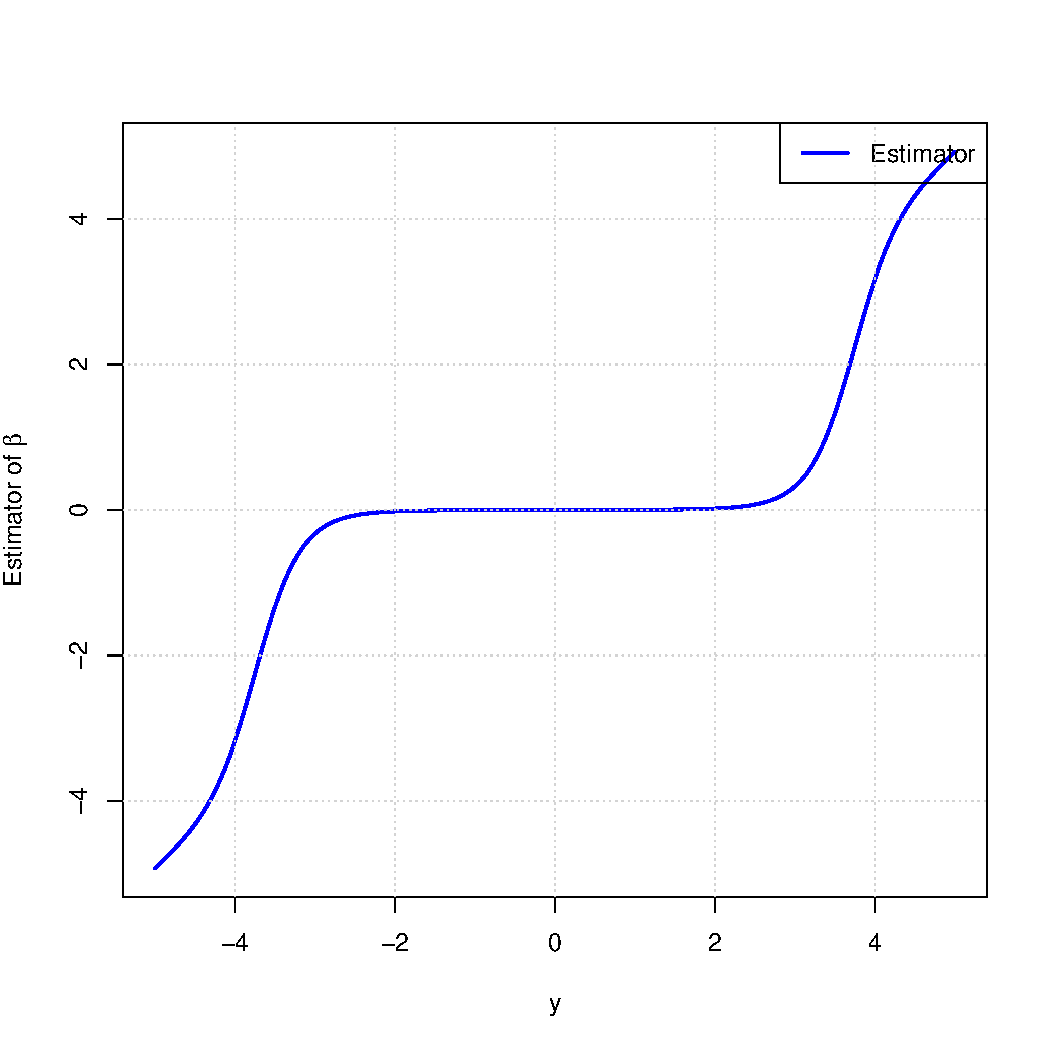
\includegraphics[width=0.65\textwidth]{Images/Figures_Exercise_3/estimator_plot.pdf}
  \caption{Estimated $\beta$ for $y \in [-5, 5]$}
  \label{fig:beta_estimator}
\end{figure}
The estimator for the $\beta$-value shares similarities with one of the lines seen in Figure (\ref{fig:inv_1}), of Exercise 1d). This resemblance is notable especially for $p = 1.1$, where the optimal $\beta$ tends to be 0 for $y \in (-1, 1)$, though the central region of Figure (\ref{fig:beta_estimator}) is wider. An assumption on the trend of Figure (\ref{fig:beta_estimator}) could suggest that increasing $\gamma$ from 1, in Exercise 1d), would generate an optimal $\beta$ more similar to the one seen above.
\nssection{c.)}
\emph{For the dataset in} \texttt{sparseDataWithErrors.dat}, \emph{evaluate the estimator using the
values $p = 0.9$, and $\tau^2 = 80$. Compare the result with 1.e, also in terms of residual
sum of squares.}  \spaze
\textbf{Solution:} \spaze
The implementation can be found in Appendix \ref{appendix:b}, from code listings (\ref{lst:residual}). It produces the following output:
\begin{align*}
    e_{\hat{\beta}_{\text{mix}}} = 108.0825
\end{align*}
In comparison to the estimates from Exercise 1.e, the $\hat{\beta}_{\text{mix}}$ estimator proves to be the most optimal, by a clear margin.